%--------------------------------------------------------------
\section{Plano de testes}
%--------------------------------------------------------------
Segundo \citeonline{Polo:2020}, por definição, os testes de \textit{software} visam assegurar que um sistema/programa atenda às necessidades dos seus usuários, assim como também permitem descobrir defeitos no funcionamento antes de disponibilizá-lo para uso. Na realização dos testes, segundo \citeonline{SOMMERVILLE:2019}, são usados dados artificiais para a sua execução.

\begin{citacao}
Os resultados dos testes são verificados para descoberta de erros, anomalias ou informações não funcionais sobre a sua execução, por exemplo, análise de desempenho, utilização de memória, etc. \cite{Polo:2020}
\end{citacao}

Considerando os apontamentos dos autores, e de modo a garantir um bom funcionamento do sistema \gls{ifriends} além de prevenir eventuais erros, foi planejado a realização de testes considerados necessários. Dessa forma, esta seção visa apresentar os testes aplicados no sistema \gls{ifriends}.

%--------------------------------------------------------------
\subsection{Testes unitários}
%--------------------------------------------------------------
Segundo \citeonline{SOMMERVILLE:2011}, por testes unitários se compreende o processo de testar componentes de programa, sendo eles métodos ou classes de objeto. Funções individuais ou métodos são os tipos mais simples de unidades. Seus testes devem ser chamados de para essas rotinas sob diferentes parâmetros. O autor ainda complementa dizendo: 

\begin{citacao}
Quando você está testando as classes de objeto, deve projetar os testes para fornecer uma cobertura de todas as características do objeto. Isso significa que você deve: testar todas as operações associadas ao objeto, definir e verificar o valor de todos os atributos associados ao objeto e colocar o objeto em todos os estados possíveis, o que significa simular todos os eventos que causam mudanças de estado
\cite{SOMMERVILLE:2011}.
\end{citacao}

Dessa forma, para o sistema \gls{ifriends}, cada novo método será feito pensando na criação dos testes unitários, de modo a também facilitar, posteriormente, seu planejamento. Os testes serão construídos efetivamente sempre após a criação de seus respectivos métodos ou classes, ou seja, após criar um método de cadastrar pergunta será feito o teste para verificar se todas as funcionalidades estão implementadas corretamente.

Além disso, considerando os apontamentos realizadas por \citeonline{StefanBechtold2021Apr} foi escolhido o \gls{JUnit} 5 como facilitador para execução dos testes automatizados na linguagem Java. Segundo a documentação do \gls{JUnit}, o \gls{framework} possui vários métodos para facilitar a verificação dos resultados, eles fazem parte da classe \textit{Assertions}, e funcionam através de anotações ``@Test'' para dizer ao sistema que o que está abaixo da anotação é um método ou uma classe de teste. O escopo sempre possui três divisões, sendo elas: cenário, que visa a preparação dos dados a serem testados; ação, que se refere ao que o teste deve executar, e a verificação, para conferir se o teste foi realizado conforme planejado.

A \autoref{exemplo teste} é um exemplo da estrutura de um teste, sendo este criado para o testar o método de salvar um usuário no banco de dados:

\begin{figure}[htb]
\centering
\caption{\label{exemplo teste} Teste na API}
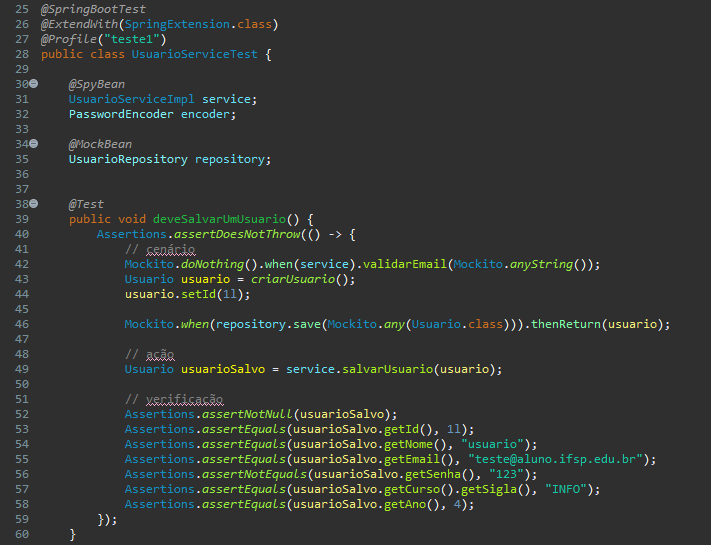
\includegraphics[width=1\textwidth]{anexos/Imagens_Testes/API_teste.png}
\fonte{os autores}
\end{figure}
\FloatBarrier

Conforme mostrado na \autoref{exemplo teste}, é possível visualizar as anotações ``@SpyBean'' e ``@MockBean'', eles são responsáveis por dizer ao \gls{SpringBoot} quais classes ele deve gerenciar e trazer para dentro do seu próprio contexto. Com a anotação ``@Profile'' é possível definir qual arquivo de propriedades será utilizado, no caso da \autoref{exemplo teste} é o arquivo que contém as configurações para o banco de dados teste.

Já para a cobertura de testes unitários está sendo utilizado o \acs{jacoco}. De acordo com sua documentação, a tecnologia oferece recursos integráveis com o \gls{JUnit}, e o \gls{Eclipse}, \acs{ide} utilizada para construção da \acs{api}. A \autoref{grafico de testes} mostra o gráfico de cobertura de testes, realizado para a classe serviço de pergunta do \gls{ifriends}:

\begin{figure}[htb]
\centering
\caption{\label{grafico de testes} Cobertura de testes}
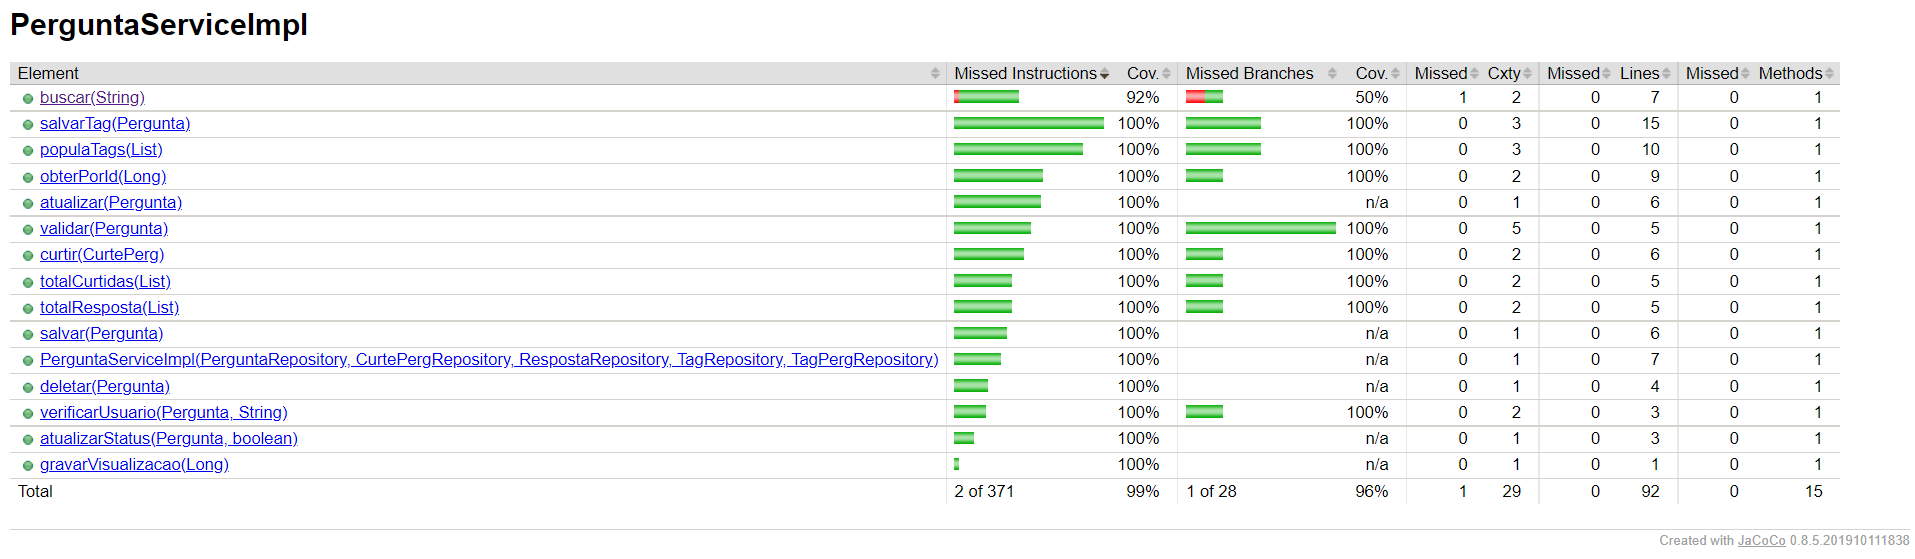
\includegraphics[width=1\textwidth]{anexos/Imagens_Testes/API_grafico-testes.png}
\fonte{os autores}
\end{figure}
\FloatBarrier

Após a observação feita do gráfico na \autoref{grafico de testes}, a segunda coluna é possível saber a porcentagem total do percurso testado por cada método; a terceira coluna mostra todas as operações testadas, e o restante das colunas mostram a quantidade de operações, linhas e métodos da classe.

%--------------------------------------------------------------
\subsection{Testes de usabilidade}
%--------------------------------------------------------------
Na parte de usabilidade, a equipe definiu que, primeiramente, será validada a interface de usuário, verificando se o sistema segue uma coerência baseada nas 10 heurísticas de Nielsen, ou seja, será um teste feito inicialmente pelos próprios desenvolvedores e conforme a frequência de entregas. Ainda para a interface, conforme os requisitos da disciplina,  o sistema deve ser inserido em um validador de interfaces ainda não definido. 

Posteriormente, será utilizada uma técnica de caixa preta para a preparação de teste de usabilidade, com a criação de cenários de teste, contando com a atuação de pelo menos 10 estudantes, que objetivem medir o desempenho, a precisão, a lembrança e a “resposta emocional” entre a interação do usuário com o sistema. As descrições de tais cenários estão em fase de planejamento, porém, a equipe também deseja realizar uma pesquisa de satisfação geral ao final dos testes, para verificar a satisfação geral do cliente com relação ao sistema desenvolvido.
